\scanpage{75}
puisse, pour tt $x$, choisir $y\in\overline{\{x\}}\cap Y$ tel que $k(y)$ soit \uline{fini}. \inserted{(c'est le cas si $A/J$ de type fini sur $\mathbf Z$).} Alors par l'argument précédent, on est ramené au cas d'un \deleted{anneau de val. discrète} \inserted{localisé complété de} $X$ en $y$, \deleted{\unsure{donc }Y_0\unsure{\text{ en }y}}, donc $X$ local complet, de pt fermé $y$, de $k(y)$ fini. Alors $X-Y$ est de Jacobson, donc tte composante connexe de $X-Y$ a un pt $z$ tel que $\dim\overline{\{z\}}=1$, \uline{Soit} $Z=\overline{\{z\}}$ et $\unsure{\text{son}}$ l'adhérence dans $X$. Cela nous ramène, \deleted{\unsure{par un théorème}} quitte à remplacer $X$ par $Z$, au cas où $X$ local complet de dim 1, et en normalisant, au cas où $X$ est \inserted{le spectre d'} un anneau de valuation discrète $V$ à corps résiduel fini, $Y$ pt fermé. L'énoncé envisagé correspond alors à un homo de modules sur $\pi=\operatorname{Gal}(\overline K/K)$, ext. de $\pi_0\simeq\deleted{\unsure{\mathbf Z}}\operatorname{Gal}(\overline k/k)$ \inserted{$=\widehat{\mathbf Z}$} par le grpe d'inertie $I$.

\deleted{On peut supposer $T\simeq\mathbf G_{mk}^{r}$ (par extension résiduelle finie) et $T_\ell(\widetilde T)|U$ correspond à
\[
\deleted{T_\ell(\overline K^*)\simeq T_\ell(\overline k^*)}\quad (\widetilde{T_\ell(\mathbf G_{mk})}|U)^r\simeq T_\ell(\mathbf G_{m\overline K})^r\simeq T_\ell(\overline K^*)^r,
\]
comme module sur $\deleted{\mathbf Z_\ell}\pi_0$. D'autre part, pour $S$ on $T_\ell(S)$ \unsure{correspond}}
\figure{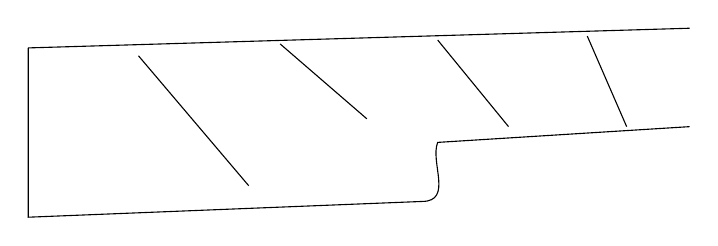
\begin{tikzpicture}[x=1cm,y=1cm]
\draw (0,2.3)--(8.4,2.55);\draw (0,2.3)--(0,.15)--(5,.35) .. controls (5.4,.35) and (5.1,.85) .. (5.2,1.1)--(8.4,1.3);
\draw (1.4,2.2)--(2.8,.55);\draw (3.2,2.35)--(4.3,1.4);\draw (5.2,2.4)--(6.1,1.3);\draw (7.1,2.45)--(7.6,1.3);
\end{tikzpicture}}
L'accouplement sur $U$, comme $X$ normal, provient d'un accouplement
\[
T_\ell(S)\times T_\ell(T)\mathbin{-}T_\ell(\mathbf G_{mk}).
\]
Donc dans ce cas on est ramené au

\uline{Lemme} Soit $k$ un corps fini, $S,\unsure{T'|T}$ deux grpes alg. commutatifs sur $k$, \deleted{dont le second est un tore} \inserted{où $T$ de t. mult.}. Alors tt. accouplement
\[
T_\ell(S)\times T_\ell(T)\mathbin{-}T_\ell(\mathbf G_m)
\]
est identiquement nul.
\margin{74}
